\chapter{The Sequence Memoizer} \label{chap:seqMem}

\todo[inline]{Sequence Memoizer section}

\section{The Theory}

The Sequence Memoizer, like the model in Chapter \ref{chap:HierarchicalDirichletModel}, uses a hierarchical model. However, instead of Dirichlet processes, it instead uses Pitman-Yor processes. These are described in more detail in Section \ref{sec:PitmanYor}.

If $\Sigma$ is the set of all possible symbols, the probability of the symbol $s$ following a context $\boldsymbol{u}$ is given in Equation \ref{eq:SM1}, where $N(s)$ is the number of occurrences of $s$ in a sequence $\boldsymbol{x}$ and $G$ is a discrete distribution over $\Sigma$. $G_{\boldsymbol{u}}$ is a conditional distribution because the probability of $s$ depends on the context $\boldsymbol{u}$.

\begin{equation}
G_{\boldsymbol{u}}(s)=\frac{N(\boldsymbol{u}s)}{\sum_{s' \in \Sigma}N(\boldsymbol{u}s')}
\label{eq:SM1}
\end{equation}

\subsection{Power Law Scaling and the Pitman-Yor Process}\label{sec:PitmanYor}

Natural language follows a power law scaling. This means that there are a large number of words that appear very infrequently and a small number of words that occur very often. The maximum likelihood estimation given in Equation \ref{eq:SM1} will perform well for the frequently occurring symbols, but not for the rare ones. This was initially discussed in Section \ref{sec:smoothing}, which implemented smoothing to counteract the problem. However, a Pitman-Yor prior follows the power law properties of natural language much more accurately.

The Pitman-Yor process (PYP), $G=\{G(s)\}_{s\in\Sigma}$, has three parameters. These are the base distribution, $G_{0}=\{G_{0}(s)\}_{s\in\Sigma}$, (mean of PYP and prior on frequency of each symbol), the discount parameter, $\alpha$, which is between 0 and 1 (affect exponent of power law), and the concentration parameter, $c$, (affects variability around $G_{0}$). When $\alpha=0$, the PYP becomes the Dirichlet process. A PYP with discount parameter $\alpha$ and prior $G_{0}$ is written $G\sim\mathcal{PY}(\alpha,G_{0})$ (we assume in this project that $c=0$).



%\subsection{Pitman-Yor Processes}\label{sec:PitmanYor}

\subsection{Inference}

As before, we want to know that probability that a symbol $s\in\Sigma$ occurs next. This is given by Equation \ref{eq:SM2}, where $\mathbb{E}$ is expectation with respect to the posterior $P(G|\boldsymbol{x})$. This expectation can be computed as in Equation \ref{eq:SM3}, where $N(s)$ is the count of symbol $s$ and $M(s)$ is another set of random counts satisfying $1\leq M(s")\leq N(s')$ if $N(s')>0$ and $M(s')=0$ otherwise. This implements a form of smoothing, as each count $N(s)$ is reduced by $\alpha M(s)$, with the total amount subtracted distributed across all symbols in $\Sigma$ proportionally to their probability under $G_{0}$.

\begin{equation}
P(\boldsymbol{x}_{T+1}=s|\boldsymbol{x})=\int P(\boldsymbol{x}_{T+1}=s|G)P(G|\boldsymbol{x})dG=\mathbb{E}[G(s)]
\label{eq:SM2}
\end{equation}

\begin{equation}
\mathbb{E}[G(s)]=\mathbb{E}\left[\frac{N(s)-\alpha M(s)+\sum_{s'\in\Sigma}\alpha M(s')G_{0}(s)}{\sum_{s'\in\Sigma}N(s')}\right]
\label{eq:SM3}
\end{equation}

\subsection{Hierarchical Pitman-Yor Processes}
Similarly to Chapter \ref{chap:HierarchicalDirichletModel}, we employ the use of hierarchical processes. In these case, these are hierarchical PYPs (HPYP). We denote the empty context as $\epsilon$ and the parent of a context $\boldsymbol{u}$ (i.e. $\boldsymbol{u}$ with the first symbol from the left removed) as $\sigma(\boldsymbol{u})$. These give Equations \ref{eq:SM4a}-\ref{eq:SM4c}.

\begin{subequations}
\label{eq:SM4}
\begin{align}
G_{\epsilon}&~\sim\mathcal{PY}(\alpha_{0},G_{0}) \label{eq:SM4a}
\\
G_{\boldsymbol{u}}|G_{\sigma(\boldsymbol{u})}&\sim\mathcal{PY}(\alpha_{|\boldsymbol{u}|},G_{\sigma(\boldsymbol{u})})\ \ \ \ \text{for all }\boldsymbol{u}\in\frac{\Sigma_{n}^{*}}{\epsilon} \label{eq:SM4b}
\\
x_{i}|\boldsymbol{x}_{i-n:i-1}=\boldsymbol{u},G_{\boldsymbol{u}}&\sim G_{\boldsymbol{u}}\ \ \ \ \text{for }i=1,...,T \label{eq:SM4c}
\end{align}
\end{subequations}

The empty context has prior $G_{0}$ and discount $\alpha_{0}$ (Equation \ref{eq:SM4a}) and any context $\boldsymbol{u}$, given its parent $\sigma(\boldsymbol{u})$, has prior $G_{\sigma(\boldsymbol{u})}$ and discount $\alpha_{|\boldsymbol{u}|}$ (Equation \ref{eq:SM4b}). The distribution over each symbol $x_{i}$ in $\boldsymbol{x}$, given that its context $\boldsymbol{u}$ consists of the previous $n$ symbols $\boldsymbol{x}_{i-n:i-1}$, is $G_{\boldsymbol{u}}$ (Equation \ref{eq:SM4c}).

\todo[inline]{Re-word}


\section{Suffix Trees} \label{sec:suffixTrees}

The strings occurring in the training corpus can be stored most efficiently in a suffix tree. These are best explained by means of an example. A simple suffix tree is built up by considering each suffix of a string individually (a suffix being any substring where the last symbol is the end of the original string - i.e. for the word "the", the possible suffixes are "e", "he" and "the"). A tree is then built up starting with the shortest suffix, then the next shortest etc. Any common substrings encountered cause the tree to branch. Construction of the suffix tree for "mississippi" is detailed below. Note that the symbol "\$" denotes the end of the word.

\qtreecenterfalse

1.\ \ \ \ \ \ \ \ \ \Tree [.$\bullet$  i\$ ]\ \ \ \ \ \ \ \ \ \ \ \ 2.\ \ \ \ \ \ \Tree [.$\bullet$ i\$ pi\$ ]\ \ \ \ \ \ \ \ \ \ \ \ 3.\ \ \ \ \ \ \Tree [.$\bullet$ i\$ [.p i\$ pi\$ ] ]\ \ \ \ \ \ \ \ \ \ \ \ 4.\ \ \ \ \ \ \Tree [.$\bullet$ [.i \$ ppi\$ ] [.p i\$ pi\$ ] ]
\\
\\
 5.\ \ \ \ \ \ \ \ \Tree [.$\bullet$ [.i \$ ppi\$ ] [.p i\$ pi\$ ] sippi\$ ]\ \ \ \ \ \ \ \ \ \ \ 6.\ \ \ \ \ \ \ \ \Tree [.$\bullet$ [.i \$ ppi\$ ] [.p i\$ pi\$ ] [.s ippi\$ sippi\$ ] ]
\qtreecentertrue
\\
\\
7.\ \ \ \ \Tree [.$\bullet$ [.i \$ ppi\$ ssippi\$ ] [.p i\$ pi\$ ] [.s ippi\$ sippi\$ ] ]
\\
\\
8.\ \ \ \ \Tree [.$\bullet$ [.i \$ ppi\$ ssippi\$ ] [.p i\$ pi\$ ] [.s [.i ssippi\$ ppi\$ ] sippi\$ ] ]
\\
\\
 9.\ \ \ \ \Tree [.$\bullet$ [.i \$ ppi\$ ssippi\$ ] [.p pi\$ i\$ ] [.s [.i ppi\$ ssippi\$ ] [.si ppi\$ ssippi\$ ] ] ]
\\
\\
10.\ \ \ \ \Tree [.$\bullet$ [.i \$ ppi\$ [.ssi ppi\$ ssippi\$ ] ] [.p pi\$ i\$ ] [.s [.i ppi\$ ssippi\$ ] [.si ppi\$ ssippi\$ ] ] ]
\\
\\
11.\ \ \ \ \Tree [.$\bullet$ [.i \$ ppi\$ [.ssi ppi\$ ssippi\$ ] ] [.p pi\$ i\$ ] [.s [.i ppi\$ ssippi\$ ] [.si ppi\$ ssippi\$ ] ] mississippi\$ ]

\subsection{The Chinese Restaurant Process}

The Chinese Restaurant Process (CRP) is commonly used in language modelling. Imagine a Chinese restaurant with an infinite number of tables. At a particular time, a new customer may choose to sit either at an existing table, or at a new unoccupied table. In our case, tables are labelled with symbols. There can be more than one table with a given symbol. Each symbol in a corpus can either be generated from the base distribution (equivalent to seating a customer at a new table)... 

If $n$ customers are already seated giving $K_{v}$ tables being occupied, the probabilities of the next customer sitting at an occupied tables or choosing a new table are given by Equations \ref{eq:CRPExisting} and \ref{eq:CRPNew} respectively, where $z_{v}^{n+1}$ is the table at which the customer will sit, $c_{v}^{k}$ is the number of customers sitting at the $k$\textsuperscript{th} table, $d_{v}$ is the discount parameter, $\alpha_{v}$ is the concentration parameter and the subscript $v\in V$ denotes a vertex in the graphical model.

\begin{equation}
P(z_{v}^{n+1}=k|\{z_{v}^{1}...z_{v}^{n}\})\propto c_{v}^{k}-d_{v}
\label{eq:CRPExisting}
\end{equation}

\begin{equation}
P(z_{v}^{n+1}=K_{v}+1|\{z_{v}^{1}...z_{v}^{n}\})\propto \alpha_{v}+d_{v}K_{v}
\label{eq:CRPNew}
\end{equation}

The CRP is implemented in our suffix tree representation of the training corpus as a Multi-Floor CRP (MFCRP). This says that customers in any given restaurant (indexed by vertex $v$) either must be associated with direct observations of draws from the underlying $G_{\boldsymbol{u}}$, or must have come from a table in a child restaurant. \todo[inline]{Re-word}

\subsection{Updating Our Representation of a Suffix Tree}

The suffix tree drawn in Section \ref{sec:suffixTrees} can be extended to include the CRP representation discussed above. The updated tree is constructed similarly by starting with the shortest suffix and working through suffixes with increasing length until the whole string has been drawn. The method for the word "mississippi" is as follows:

\begin{enumerate}
\item Begin with the suffix "i"
\begin{enumerate}
\item Create a branch for the empty context with a restaurant containing a table for the letter "i" with one customer
\item Add a table in the top level restaurant for the letter "i" with one customer
\end{enumerate}
\item For suffix "pi":
\begin{enumerate}
\item Create a branch for the context "i" with a restaurant containing a table for the letter "p" with one customer
\item Add a table in the top level restaurant for the letter "p" with one customer
\end{enumerate}
\item Continue with suffixes of increasing length...
\item For suffix "sippi":
\begin{enumerate}
\item There is already a branch for context "i"
\item Create a branch for the context "ppi" as a child of branch "i" with a restaurant containing a table for the letter "s" with one customer
\item Create a branch for the empty context as a child of branch "i" with a restaurant containing a table for the letter "p" with one customer
\item For the restaurant of branch "i" check that there is a table for the letter "s" with one customer and a table for the letter "p" with one customer
\end{enumerate}
\item Continue for the remaining suffixes
\end{enumerate}

The key difference in construction between this new representation and the original, simpler representation is that the first letter of the suffix being considered has a table with a customer in the deepest restaurant. Otherwise, the branch labels are very similar. The total number of customers for any letter in a given restaurant must be equal to the total number of tables in all of that restaurant's child restaurants. For simplicity, all customers have been seated at existing tables (where possible) for their letter in Figure \ref{fig:mississippiSuffixTree}, but a more comprehensive tree would have branches for all possible arrangements of customers and tables.

\begin{figure}[h!]
  \centering
  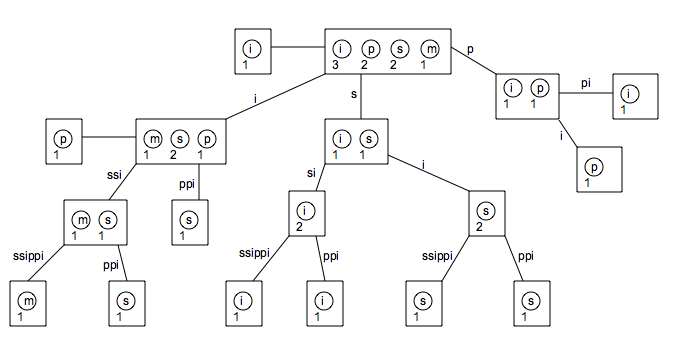
\includegraphics[width = 1\linewidth]{mississippi_suffix_tree.png}
  \caption{Suffix Tree with CRP Representation for "mississippi"}
  \label{fig:mississippiSuffixTree}
\end{figure}




\section{Prediction}